

\begin{enumerate}
	\item 
    \begin{enumerate}
        \item No, this is not possible because the original ODE has units of $\frac{mass * length}{time^2}$ for each term on the left hand side, whereas the units for the terms $2y'$ and $4y$ would have different units.

        \item The characteristic equation is $r^2+2r+4 = 0$.

        \item We expect complex roots since the discriminant of the characteristic equation is negative. The roots are $-1+i\sqrt{3}$ and $-1-i\sqrt{3}$, matching our expectation.

        \item The general, complex solution to the ODE is:
        \[
        y(t) = c_1e^{(-1+i\sqrt{3})t} + c_2e^{(-1-i\sqrt{3})t}
        \]

        \item The general, real solution to the ODE is:
        \[
        y(t) = e^{-t}[c_1\cos(\sqrt{3}t)+c_2\sin{(\sqrt{3}t)}]
        \]

        \item If we graph the solution with $c_1=c_2=1$, we get the following curve:

        \begin{figure}[h]
        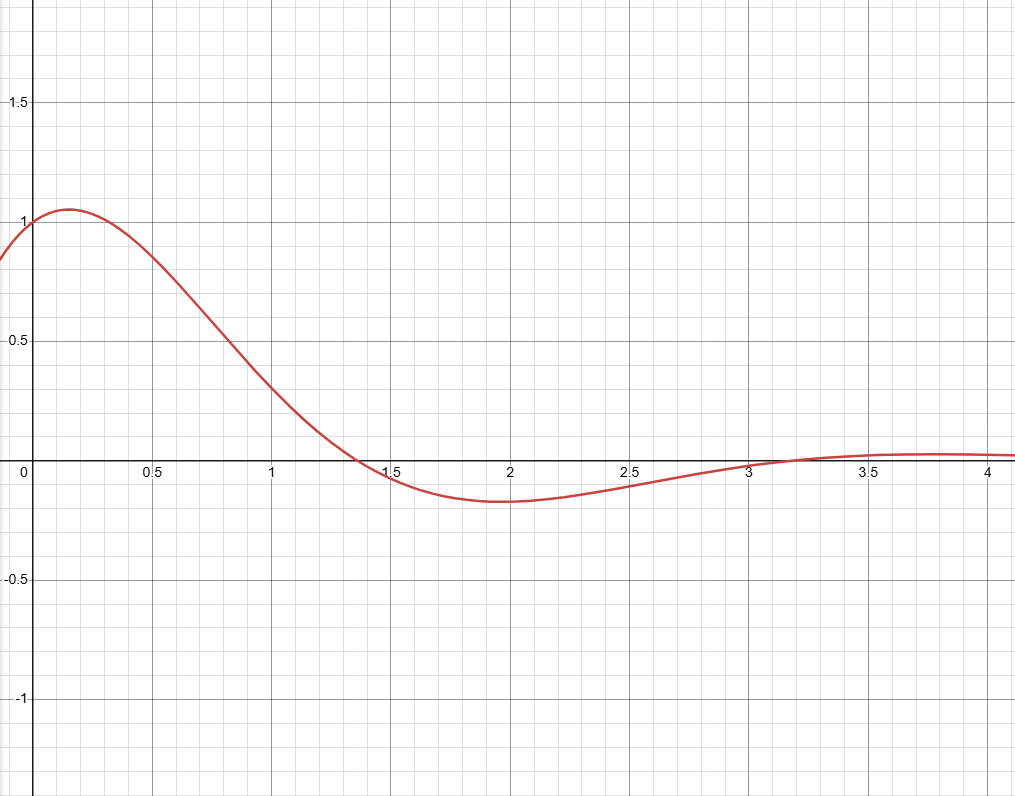
\includegraphics[width=8cm]{tutorials/Tut9_Q1.png}
        \centering
        \end{figure}

        If we were to remove the exponential factor, this would be a periodic function with a period of $\frac{2\pi}{\sqrt{3}}$ rad/s. This is what is causing the function to not be exactly periodic, so we must use the term ``quasi-periodic" instead.
    \end{enumerate}

    \item 
    \begin{enumerate}
        \item The difference between temperatures is $A - B$. Since $A'$ is proportional to this with proportionality constant 2, either $A' = 2(A- B)$ or $A' = 2(B-A)$. Since if $B > A$ means room A heats up, the second ODE is most appropriate, i.e., $A' = 2(B-A)$.

        \item Using the same argument above, we can write $B' = 2(A - B)$. However, since room B has windows, we must also add the external effect $\frac{1}{2}\sin{\frac{\pi t}{12}}$: $B' = 2(A-B) + \frac{1}{2}\sin{\frac{\pi t}{12}}$.

        \item We can derive the following:
	
    	\[
    	    A' = 2(B-A)\\
    	    \implies A'' = 2\left(B'-A'\right)\\
    	    \implies A'' = 2\left[2(A-B) + \frac{1}{2}\sin{\frac{\pi t}{12}} - A'\right]
    	\]
    	
    	Since $A' = 2(B-A)$, we can write $B = \frac{1}{2}A' + A$. Plugging this into the above yields:
    	
    	\[
    	    A'' = 2\left[2\left(A - \left(\frac{1}{2}A' + A\right)\right) + \frac{1}{2}\sin{\frac{\pi t}{12}} - A'\right]\\
    	    \implies A'' + 4A' = \sin{\frac{\pi t}{12}}
    	\]

        \item The characteristic equation is given by $r^2 + 4r = 0 \implies r_{1,2} = 0, -4$. 
	    
	    Since the roots are real, the oscillator is overdamped. Since there is a forcing function as well, the oscillator is forced. 
	    
	    In the applied context, the external forcing describes the influence of the outside temperature. The oscillator itself is a damped since, without external influence, the temperature in rooms A and B would ``balance out" over time, i.e., stabilize.
    \end{enumerate}
\end{enumerate}